\documentclass[12pt]{article}
\usepackage[utf8]{inputenc}
\usepackage{graphicx}
\usepackage{amsmath}
\usepackage{siunitx}
\usepackage{booktabs}
\usepackage[margin=1in]{geometry}

\title{Aerospace Senior Project Weekly Report}
\author{Team Gamma}
\date{Week 1 - January 21, 2025}

\begin{document}
\maketitle

\section{Week 1 Progress Report}\label{week-1-progress-report}

\subsection{Progress Made}\label{progress-made}

\subsubsection{Product Breakdown
Structure}\label{product-breakdown-structure}

\begin{itemize}
\tightlist
\item
  We began by forming an initial product Breakdown
\item
  We then used this breakdown to begin researching requirements
\end{itemize}

\subsubsection{Research Topics Summary}\label{research-topics-summary}

We began researching: - FAA Requlations on: - Runways - Hangers -
Weather conditions - Stability - Safety (fire suppresion and cabin
dimensions) - Comparable Jets - The A380 was used for many preliminary
calculations, as the largest currently operated passenger jet.

\subsubsection{Requirements}\label{requirements}

\begin{itemize}
\tightlist
\item
  Since we are designing a large transport vehicle, the 14 CFR 25
  (airworthiness standards for transport category airplanes) was used to
  determine many of the FAA requirements for the plane.
\item
  Mission requirements were also categorized.
\item
  Other ``customer requirements'' were drafted from mission requirements
  and regulations. These will be used to guide trade studies for the
  determination of design requirements.
\item
  Requirements were drafted in the following categories:

  \begin{itemize}
  \tightlist
  \item
    Stability
  \item
    Passenger loading
  \item
    Weight
  \item
    Performance
  \item
    Operational Internal Components
  \item
    Passenger components: Windows, seats, bathrooms, food preparation
  \end{itemize}
\end{itemize}

\subsubsection{Weight Calculations}\label{weight-calculations}

\begin{itemize}
\tightlist
\item
  Crew weight was found to be \textasciitilde4,818 lbs
\item
  Payload weight was found to be \textasciitilde331,660 lbs
\item
  Total weight was found to be \textasciitilde2,233,541 lbs
\end{itemize}

\subsubsection{Mission Diagram}\label{mission-diagram}

The first draft of the mission diagram was created:
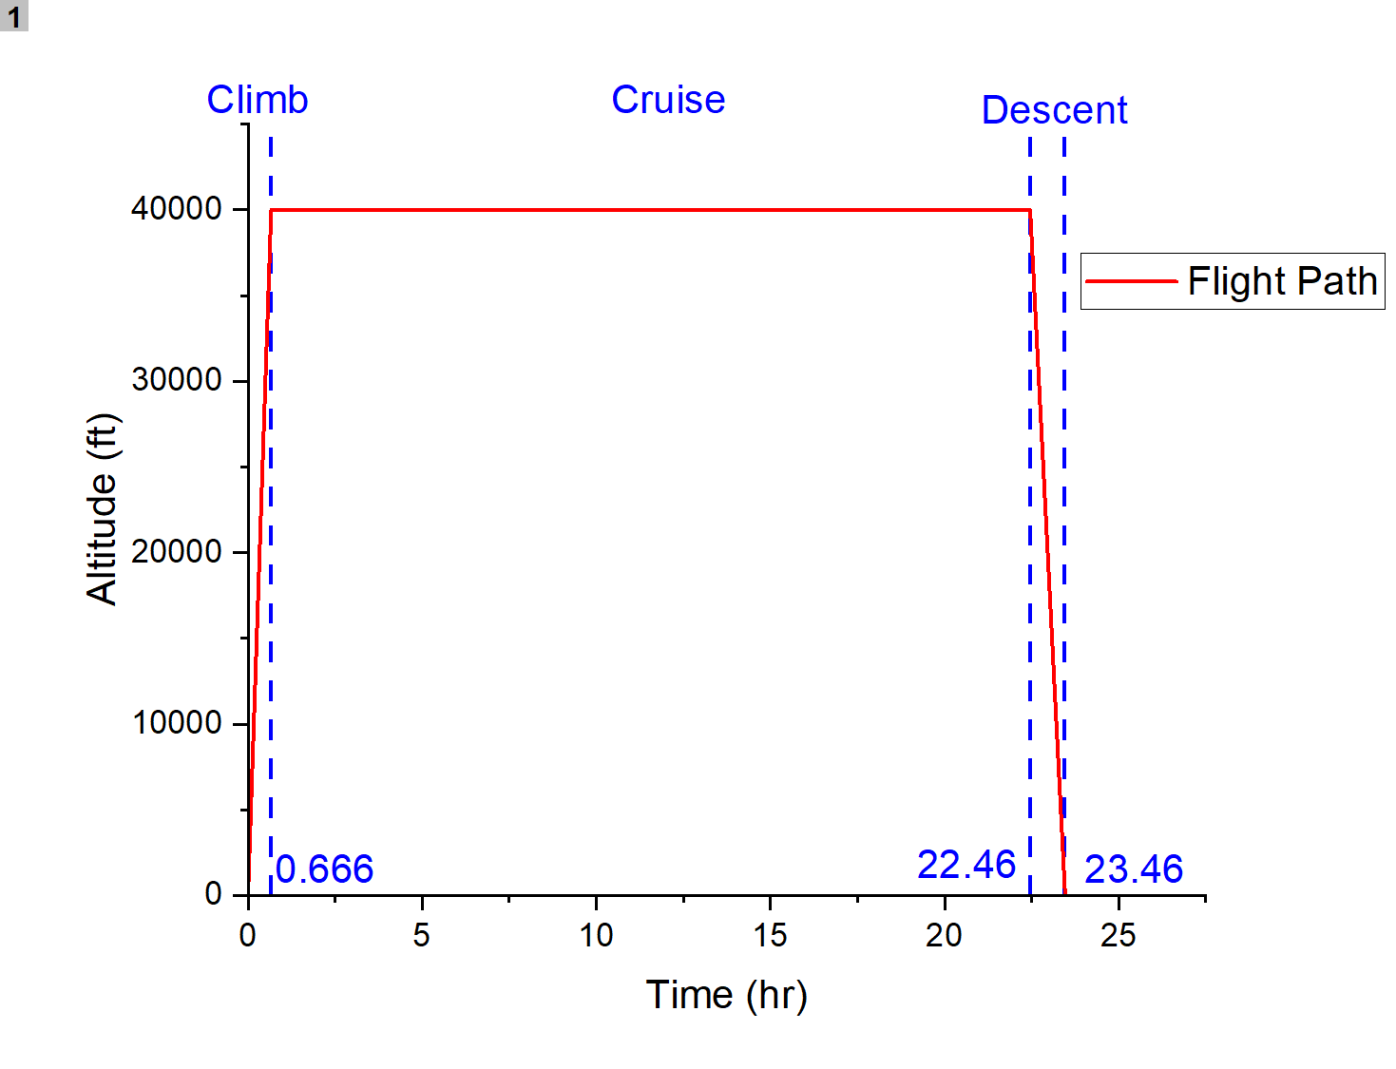
\includegraphics{../assets/week_01/mission_diagram.png}

\subsection{Next Week's Objectives}\label{next-weeks-objectives}

\subsubsection{Continued Research}\label{continued-research}

Next week, we aim to continue researching the above topics. Specific
additional research includes: - Water Storage - Takeoff thrust
determination (this will aid in specifying many engine requirements) -
Taining requirements

\subsubsection{Trade Studies}\label{trade-studies}

We aim to begin conducting the following trade studies: - Cabin and Seat
configuration - Cruise thrust requirements - Takeoff/Landing thrust
requirements - Alternative fuselage designs (double fuselage, flying
wing, double decker, etc.) - Wing geometry - Fuel Efficiencies

\end{document}

% presentation_template.tex
\documentclass{beamer}
\usetheme{Madrid}
\usecolortheme{whale}
\usepackage{graphicx}
\usepackage{amsmath}
\usepackage{siunitx}

\title{Aerospace Senior Project Progress}
\author{Team Gamma}
\date{Week 1 - January 21, 2025}

\begin{document}

\frame{\titlepage}

\frame{
\frametitle{Contents}
\tableofcontents
}

\section{Week 1 Progress Report}\label{week-1-progress-report}

\subsection{Progress Made}\label{progress-made}

\subsubsection{Product Breakdown
Structure}\label{product-breakdown-structure}

\begin{itemize}
\tightlist
\item
  We began by forming an initial product Breakdown
\item
  We then used this breakdown to begin researching requirements
\end{itemize}

\subsubsection{Research Topics Summary}\label{research-topics-summary}

We began researching: - FAA Requlations on: - Runways - Hangers -
Weather conditions - Stability - Safety (fire suppresion and cabin
dimensions) - Comparable Jets - The A380 was used for many preliminary
calculations, as the largest currently operated passenger jet.

\subsubsection{Requirements}\label{requirements}

\begin{itemize}
\tightlist
\item
  Since we are designing a large transport vehicle, the 14 CFR 25
  (airworthiness standards for transport category airplanes) was used to
  determine many of the FAA requirements for the plane.
\item
  Mission requirements were also categorized.
\item
  Other ``customer requirements'' were drafted from mission requirements
  and regulations. These will be used to guide trade studies for the
  determination of design requirements.
\item
  Requirements were drafted in the following categories:

  \begin{itemize}
  \tightlist
  \item
    Stability
  \item
    Passenger loading
  \item
    Weight
  \item
    Performance
  \item
    Operational Internal Components
  \item
    Passenger components: Windows, seats, bathrooms, food preparation
  \end{itemize}
\end{itemize}

\subsubsection{Weight Calculations}\label{weight-calculations}

\begin{itemize}
\tightlist
\item
  Crew weight was found to be \textasciitilde4,818 lbs
\item
  Payload weight was found to be \textasciitilde331,660 lbs
\item
  Total weight was found to be \textasciitilde2,233,541 lbs
\end{itemize}

\subsubsection{Mission Diagram}\label{mission-diagram}

The first draft of the mission diagram was created:
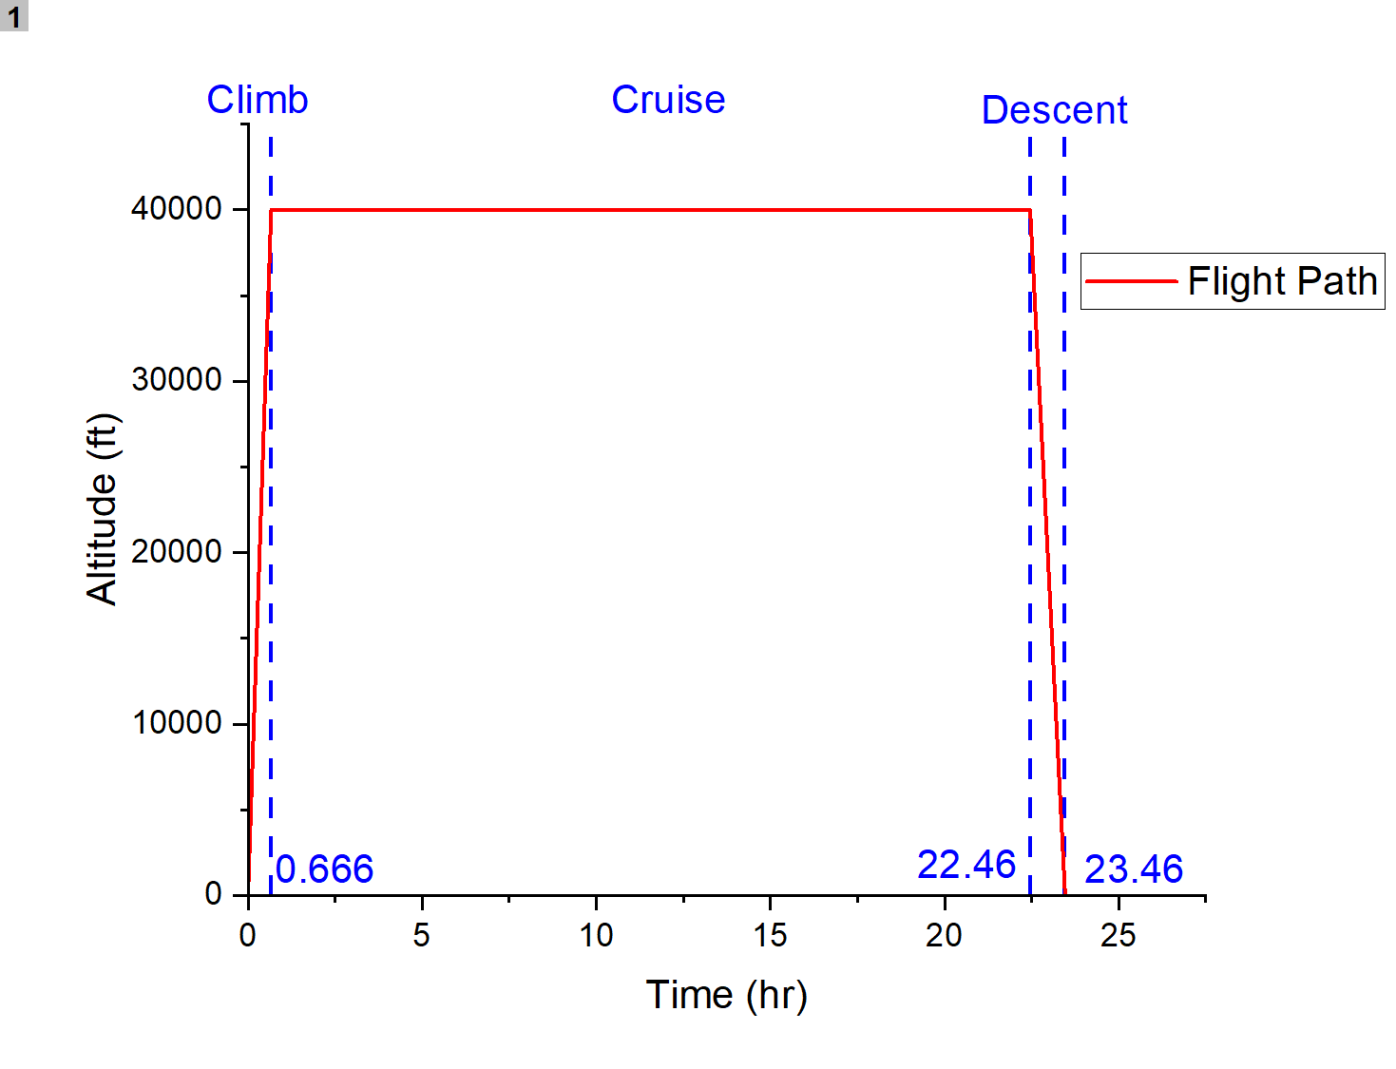
\includegraphics{../assets/week_01/mission_diagram.png}

\subsection{Next Week's Objectives}\label{next-weeks-objectives}

\subsubsection{Continued Research}\label{continued-research}

Next week, we aim to continue researching the above topics. Specific
additional research includes: - Water Storage - Takeoff thrust
determination (this will aid in specifying many engine requirements) -
Taining requirements

\subsubsection{Trade Studies}\label{trade-studies}

We aim to begin conducting the following trade studies: - Cabin and Seat
configuration - Cruise thrust requirements - Takeoff/Landing thrust
requirements - Alternative fuselage designs (double fuselage, flying
wing, double decker, etc.) - Wing geometry - Fuel Efficiencies

\end{document}
